\chapter{Numerical methods}
\label{chap-sim}

In 1949, Metropolis \cite{metropolis_monte_1949} discovers a method to compute, through Monte Carlo simulations, the expectation value of statistical quantities. If $Q$ is an observable quantity of a statistical system, such as the total energy or density of particles per site, then the expectation value is computed by weighting its value over all configurations $C$ with respect to their statistical weight. If we consider the system to be at thermodynamic equilibrium, then every configuration $C$ follows the Gibbs-Boltzmann distribution, and the mean value $<Q>$ is
\begin{align}
    <Q> = \frac{\sum_{C} Q(C) \exp(-\beta E(C))}{\sum_{C} \exp(-\beta E(C))}
\end{align}
For example, in a SOS system of size $100\times100$ - which is small compared to the thermodynamic limit as discussed in figure \ref{fig-thermo-libre} - there exist $100^{100}$ different possible configurations. In comparison, numerical simulations can explore up to $10^9$ configurations in a reasonable amount of CPU time.

Nevertheless, lattice models are well fitted for Monte Carlo simulations, where the goal is to compute is to compute such quantities. In the SOS model, all observables (and even quantities not observable such as the free energy) can be directly computed thanks to the matrix transfer in the grand-canonical ensemble. Nevertheless, as stated prior, the canonical ensemble stays out of reach of that method.

In this chapter, we start by explaining how Monte Carlo Metropolis algorithm works based upon the statistical ensemble we're interested in, at or out of equilibrium.
At last, I will give some technical considerations about optimizing numerical simulations.

This work has been made possible thanks to the Mésocentre de Calcul Intensif Aquitain (MCIA)\cite{noauthor_mesocentre_nodate}, where I've made the vast majority of the numerical simulations.
All the code I've produced can be found on Github \cite{paul_gersberg_github_2020} under Creative Commons BY 3.0 licence\footnote{\url{https://creativecommons.org/licenses/by/3.0/fr/deed.en}}. Numerical simulations where made with C++, parallelization with MPI, data treatment with Python, and some minor scripts in Bash.

%%%%%%%%%%%%%%%%%%%%%%%%%
    \section{Estimator}
%%%%%%%%%%%%%%%%%%%%%%%%%

Monte Carlo simulations explore the configurations' space in a random fashion \cite{newman_monte_1999} with a probability $p(C)$ which we will define later one. By choosing $M$ states ${C_0,...,C_M}$, the estimator $Q_M$ of $Q$ is given by
\begin{align}
    Q_M = \frac{\sum_{i=0}^M Q(C_i) p(C_i)^{-1} \exp(-\beta E(C_i))}{\sum_{i=0}^M  p(C_i)^{-1} \exp(-\beta E(C_i))}
\end{align}
The bigger the $M$, the better estimate the estimator provides for $<Q>$, up to the limit $Q_{M\to \infty} = <Q>$. If we select the configurations over which we sample the system according to the Gibbs-Boltzmann distribution $p(\nu) = Z^{-1} e^{-\beta E(C)}$, the estimator of $<Q>$ is
\begin{align}
    Q_M = \frac{1}{M} \sum_{i=0}^M Q(C_i)
\end{align}
The error over this estimate is
\begin{align}
	E(Q) = \sqrt{\frac{2 \tau}{M} (<Q^2>-<Q>^2)} 
\end{align}
This error does depend from the correlation time $\tau$ since if two states are really close in time, they would be strongly correlated, adding little information to the estimator. In practice, we just need $\frac{\tau}{M} \less 10^{-4}$ to obtain an error under $1\%$. This correlation time $\tau$ is computed through the autocorrelation function
\begin{align}
    \mC(t) = <Q(t')Q(t+t')>- <Q>^2 = \frac{1}{t}\int_0^t Q(t')Q(t+t')-<Q>^2 dt' 
\end{align}
which behaves as an exponential at long time\cite{wansleben_monte_1991}. A first order estimate of $\tau$ is thus given for
\begin{align}
	\tau = \int_0^{\infty} \mC(t)/\mC(0) dt
	\label{tau_cor}
\end{align}
Similarly, the measurement of the correlation length $\xi$ is given at first order by integration the two-point correlation function
\begin{align}
\mC(j) = \frac{1}{L'} \sum_{i=0}^{L'} <h_i h_{i+j}>-<h>^2 
\end{align}

%%%%%%%%%%%%%%%%%%%%%%%%%%%%%%
    \section{Monte Carlo Metropolis algorithm}
%%%%%%%%%%%%%%%%%%%%%%%%%%%%%%

We know want to know how to choose configurations, so all of them has the good equilibrium probability.

A dynamic for systems with a discrete configuration state can be built using Markov chains. Let the dynamic evolve in a discrete time $n$, and $p_n(C)$ the probability that the system is in configuration $C$ at time $n$. On the time step, if the system is in state $C$, it can jump to another state $C'$ with a transition probability $\rho(C\to C')$. The system at time $n+1$ thus only depends of the state at time $n$ : that's a Markovian process. The probability $p_{n+1}(C)$ to be in state $C$ at time $n+1$ is equal to the probability that the system was already in state $C$ at time $n$ and stays put with a transition probability $\rho(C\to C)$ , plus the probability that it was in state $C'$ and jumps towards $C$ with a transition probability $\rho(C'\to C)$. The master equation of such a dynamic is
\begin{align}
p_{n+1}(C) = \rho(C\to C) p_n(C) + \sum_{C'\neq C} \rho(C'\to C) p_n(C')
\end{align}
Since $\rho(C' \to C)$ is a probability, it meets the requirements 
\begin{align}
\sum_{C'} \rho(C' \to C) = 1
\label{norm}
\end{align}
Now, if the dynamics describes a system in interaction with a heat bath, the equilibrium distribution is given by
\begin{align}
p_{eq}(C) = \frac{\exp(-\beta E(C))}{Z}
\end{align}
with $Z$ the partition function. Since the equilibrium distribution is also stationary, we have
\begin{align}
p_{eq}(C) = \rho(C\to C) p_{eq}(C) + \sum_{C'\neq C} \rho(C'\to C)p_{eq}(C')
\label{p-eq-mc}
\end{align}
Another condition that we need in order to generate Gibbs-Boltmanzz states, is that it complies with detailed balance. To comply with detailed balance, the transition rate from a state to another one is equal to the rate from the reciprocal transition, which gives
\begin{align}
\sum_{C'} p(C) \rho(C \to C') = \sum_{C'} p(C') \rho(C' \to C)
\end{align}
We can show that this relation is equivalent to \cite{newman_monte_1999} 
\begin{align}
\frac{\rho(C'\to C)}{\rho(C \to C')} = \frac{p(C)}{p(C')} = \frac{\exp(-\beta E(C))}{\exp(-\beta E(C'))}
\end{align} 
By adopting the detailed balance, we easily see that the equilibrium distribution computed by Eq \eqref{p-eq-mc} gives back the Gibbs-Boltzmann distribution. 
During a Metropolis step, the transition probability of $C\to C'$ depends of the probability $g(C\to C')$ that this transition would be chosen amongst all the other possible transitions, and the acceptance rate ${A(C \to C')}$, which gives
\begin{align}
    \rho(C\to C') = g(C\to C') A(C \to C')
    \label{acceptance-mc}
\end{align}
For a lattice model site $L'$ sites, we say that a Monte Carlo time step is done when we have proceeded to $L'$ transition tries.
%%%%%%%%%%%%%%
\subsection{Glauber dynamics}
%%%%%%%%%%%%%%

In the SOS model with $L'$ sites of height comprised in $[0,L]$, the Glauber algorithm \cite{glauber_timedependent_1963} makes us chose a site $i$ at random with a uniform probability $\frac{1}{L'}$ and an integer $\alpha = \pm 1$ with probability $\frac{1}{2}$. If the configuration $C$ has the Hamiltonian $H(h_0,h_1...,h_i,...h_{L'})$, then the new generated configuration will have the Hamiltonian $H(h_0,h_1...,h_i+\alpha,...h_{L'})$.
If $\alpha=+1$, then we add a particle at site $i$, otherwise we remove one. In the case that $h_i+\alpha \not\in [0,L]$ , the generated configuration is not valid and discarded.
If the generated configuration is valid, the probability of selecting this transition is
\begin{align}
g(C\to C') = \frac{1}{2L'}
\end{align}
We thus have
\begin{align}
\frac{\rho(C\to C')}{\rho(C' \to C)} = \frac{A(C\to C')}{A(C'\to C)} = \exp(-\beta (E(C')-E(C'))
\end{align}
Is it possible to choose any acceptance rate $A(C\to C')$ which satisfies detailed balance. A Metropolis algorithm is an algorithm which has the following acceptance rate
\begin{align}
A(C\to C') = \begin{cases} \exp(-\beta (E(C')-E(C)) &\text{ if } E(C')-E(C) \greater 0 \\
1 &\text{ otherwise} \end{cases}
\label{taux-transition-metropolis}
\end{align}
In practice, if $\Delta E \greater 0$, we randomly choose an integer uniformly in $r\in[0,1]$. If $r\less A(C\to C') $ then the transition is accepted. Otherwise, the transition is rejected and the system stays in the configuration $C$.

Since $\sum_i h_i$ is not conserved over time, Glauber dynamics corresponds to model A.

\begin{figure}
\centering
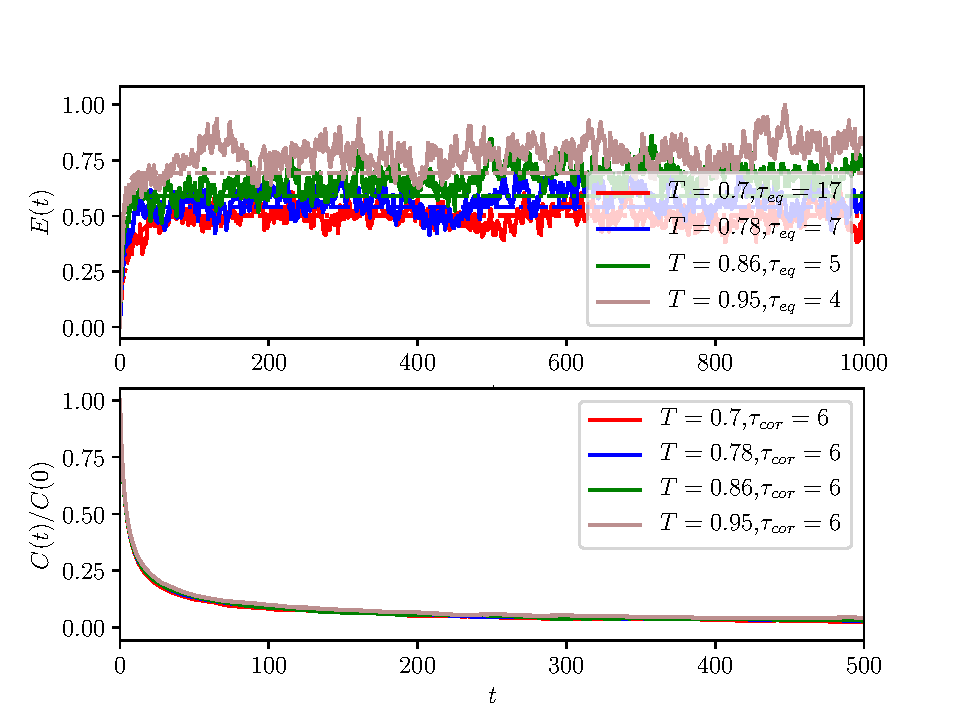
\includegraphics[scale=1]{numerical/sos-glau-eq-cor.pdf}
\caption{Plot of the energy per site (top) and the autocorrelation function (bottom) with Glauber dynamics from an initial state where $h_i=0$, for different temperatures.}
\label{eq-glau}
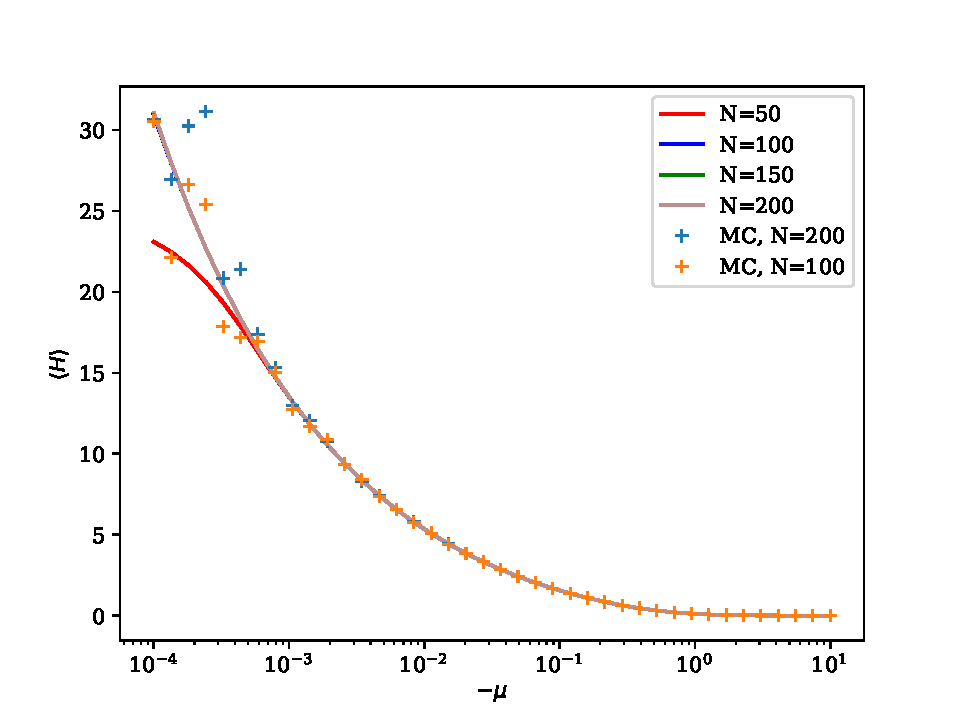
\includegraphics[scale=0.5]{numerical/comp-mc-tm-mu.pdf}
\caption{Mean height value per site with respect to $\mu$ different system size $L$ both by Glauber dynamics and diagonalization of the transfer matrix (which has already been shown in Fig \ref{hauteur-mu}) for $\beta=1$ and $L' = 256$.}
\label{tm-mc-equalt} 
\end{figure}
The energy difference between two configurations is
\begin{align}
	\Delta E &= |h_{i-1}-(h_i + \alpha)| + |h_{i+1}-(h_i + \alpha)| - |h_{i-1}-h_i| - |h_{i+1}-h_i|  
\end{align}
It is not needed to compute the total height at each time step. We can stock $\sum_i h_i$ in a variable that is updated each time a transition is accepted by
\begin{align}
    <h>_{M+1} = <h>_M + \alpha
\end{align}
We can do the same for $\sum_i h_i^2$, which gives us the interface's width, or the total energy of the system with $\sum_i |h_i - h_{i+1}$.

In order to accelerate the equilibration process, we can directly start from the total height computed by the transfer matrix. We then get the equilibrium time by looking at $E(t)$. It is better practice to choose study the equilibration time by taking the total energy instead of the magnetization, since without external potential, the interface is delocalised and magnetization is only bounded by the boundary conditions. In Fig \ref{eq-glau}, we show the energy with respect to time and the autocorrelation function of the system in absence of chemical potential from a ground state $h_i=0$ for all $i$. The very small correlation and equilibration times means that numerical simulations reach the equilibrium distribution after $10^3$ MC steps, and that only $10^7$ MC steps will give accurate results.

In the SOS model, we expect to have the results from the Glauber dynamics to be exactly the same as the transfer matrix method, as shown in Fig \ref{tm-mc-equalt}. Since the interface is not localised for small $\mu$, even though we reach thermal equilibrium fast, the mean height  fluctuates a lot, making its measurement irrelevant in the delocalised limit. Since we can get exact results from the transfer matrix, the Glauber dynamics presents little interest for SOS models in the grand-canonical ensemble. Nevertheless, because there does not exist a transfer matrix formulation of the canonical ensemble, Monte Carlo simulations become interesting.

%%%%%%%%%%%%%%
\subsection{Kawasaki dynamics}
%%%%%%%%%%%%%%

Now we would like to have an algorithm for the canonical ensemble, where the total height stays constant. In the Kawasaki's algorithm \cite{kawasaki_diffusion_1966}, we randomly choose a site $i$ with probability $\frac{1}{L'}$, and one of its two neares neighboors $i-1$ or $i+1$ with probability $\frac{1}{2}$. For example, if we take the neighboor site $i-1$ (it holds the same for the site $i+1$), we generate a new configuration with Hamiltonian $H(h_0,...,h_{i-1}+1,h_i-1,...h_{L'})$, where we have taken a particle from site $i$ to diffuse it to the other site.
The selection probability is
\begin{align}
g(C\to C') = \frac{1}{2L'}
\end{align}
We also chose the same acceptance rate as in Glauber's dynamics \eqref{taux-transition-metropolis}.

Here, the total height is obviously conserved. In the case that we transfer a particle to site $i$ to site $i+1$, the energy difference is
\begin{align}
\Delta E &= |h_{i-1}-(h_i - 1)| + |h_{i+1} + 1 -(h_i- 1)| + |h_{i+1} + 1-(h_{i+2} )| \nn
& - \left( |h_{i-1}-h_i| + |h_{i+1} -h_i| + |h_{i+1}-h_{i+2}| \right)
\end{align}

\begin{figure}[t]
\centering
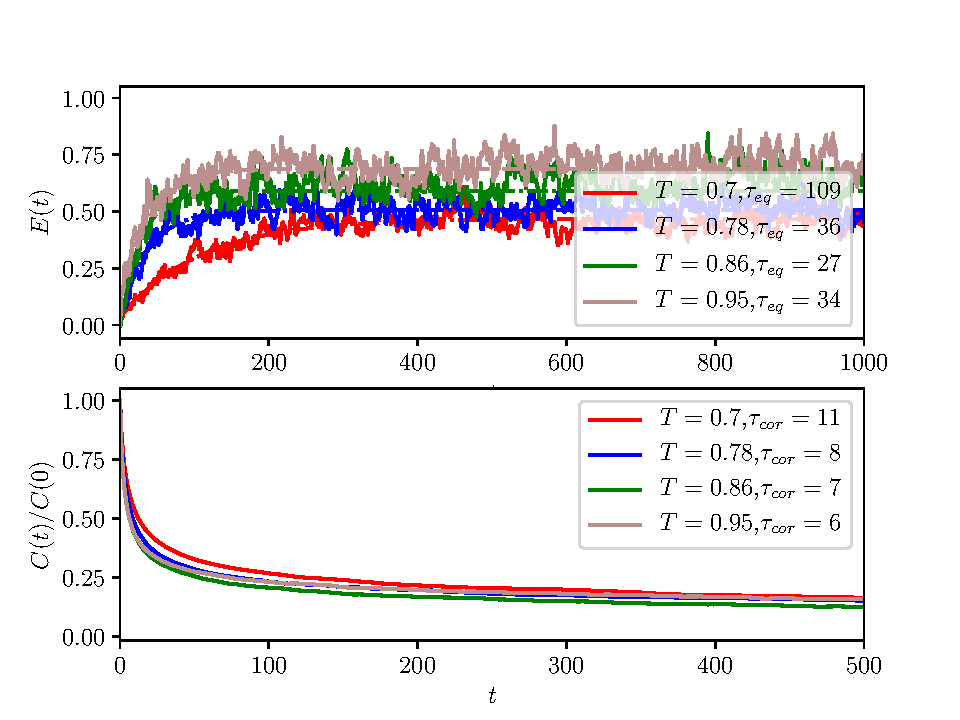
\includegraphics[scale=1]{numerical/sos-kaw-eq-cor.pdf}
\caption{Plot of the energy per site (top) and the autocorrelation function (bottom) with Kawasaki dynamics from an initial state where $h_i=0$, for different temperatures.}
\label{eq-kaw}
\end{figure}
In Fig \ref{eq-kaw}, we remark that both the equilibration and the correlation time are larger than for non-conserved dynamics, which is normal since the correlation length during coarsening goas as $t^\frac{1}{2}$ in model A and as $t^\frac{1}{3}$ in model B. Nevertheless they are of the same order of magnitude, which means that numerical simulations will take the same CPU time.

This dynamic describes the diffusion of particles at the interface. It is thus possible to add some hydrodynamic flow which breaks equilibrium. Since we have supposed that our configurations obeys the Gibbs-Boltzmann distribution, the Metropolis method stays pertinent if we assume that the dynamic is slow compared to the heat exchange with the reservoir.

%%%%%%%%%%%%%%%%%%% 
\section{Computing size dependent free energy}
%%%%%%%%%%%%%%%%%%% 

%%%%%%%%%%%%%%%%%%% 
\subsection{The Layer method}
%%%%%%%%%%%%%%%%%%%  

\begin{figure}
\begin{minipage}[t]{0.32\linewidth}
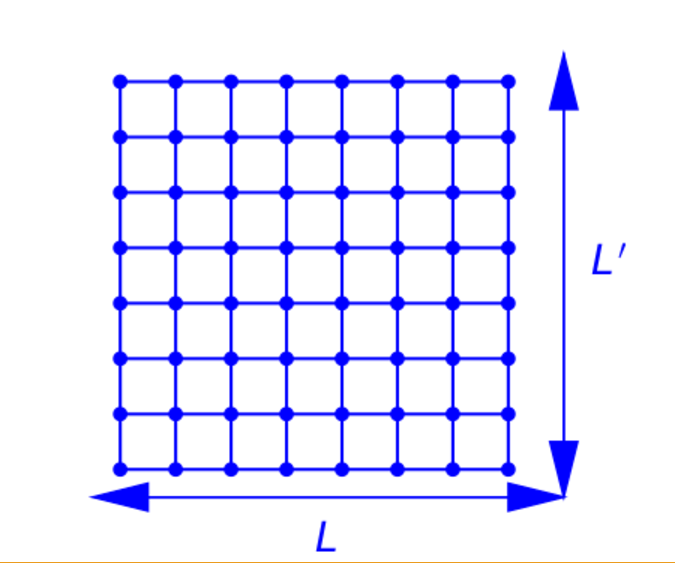
\includegraphics[width=\linewidth]{numerical/cross-h0.pdf}
\caption*{$H_0$}
\end{minipage}
\begin{minipage}[t]{0.32\linewidth}
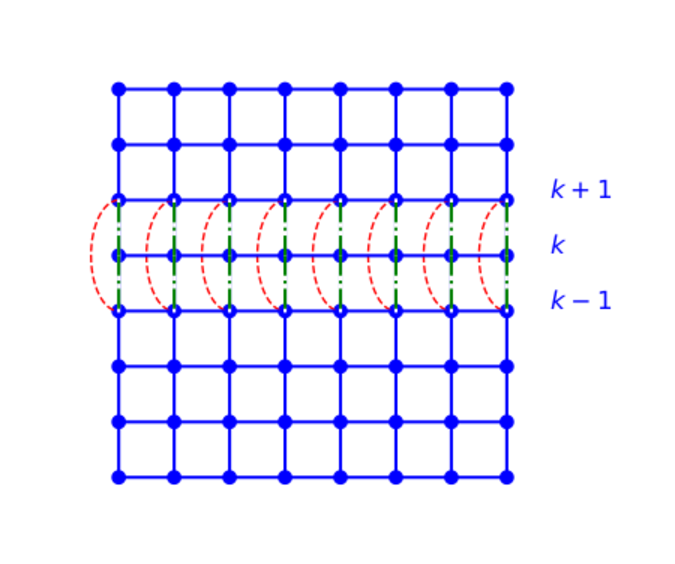
\includegraphics[width=\linewidth]{numerical/cross-hlambda.pdf}
\caption*{$H(\lambda)$} 
\end{minipage}
\centering
\begin{minipage}[t]{0.32\linewidth}
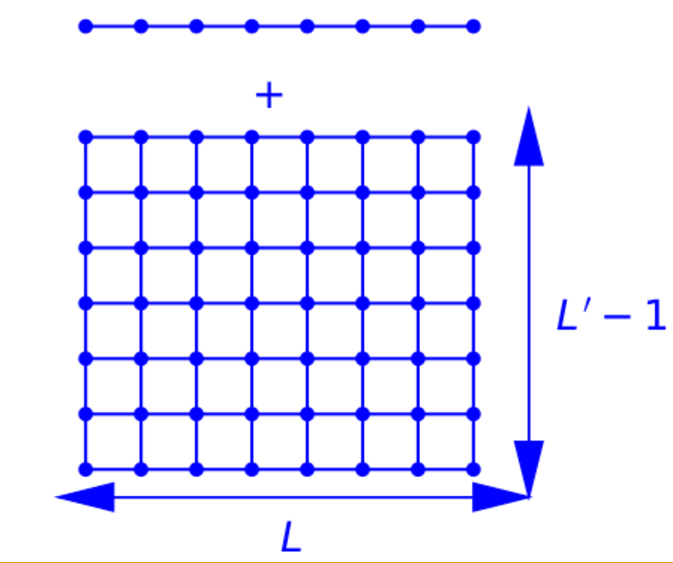
\includegraphics[width=\linewidth]{numerical/cross-h1.pdf}
\caption*{$H_1$}
\end{minipage}
\caption{Progessive decoupling of the $k$-th layer of the system in order to compute the freen energy through the Crossover Hamiltonian. Blue bonds have an energy of $\beta J$, red ones an energy of $\lambda \beta J $ and the green ones an energy of$ (1-\lambda) \beta J$. Reproduction 2D of \cite{ vasilyev_universal_2009}.}
\label{decouplage}
\end{figure}

It is not possible to compute from Monte Carlo simulations the free energy of a system, since it is not a derivative of the partition function. However, we can compute its derivative with respect to the system. This is useful to compute 
{\color{brown} As detailed later in Sec \ref{sec-casimir}, the total free energy of the confined system has a bulk and a singular part
\begin{align}
    F(t,h,L) = L'^2 \left( L f_{bulk} + \beta^{-1} f_{ex} \right)
    \label{dec-free-ene}
\end{align}
where $f_{bulk}$ is a bulk term, and $f_{ex}$ the excess free energy due to boundary conditions. 
The thermodynamic force per unit area is defined as 
\begin{align}
p(t,h,L) = - \frac{1}{L'^2 }\frac{\partial F}{\partial L} = - f_{bulk} - \beta^{-1} \frac{\partial f_{ex}}{\partial L}
\label{casmir-mc}
\end{align}
We see that this force is composed of a bulk term and an excess term, which is the Casimir force, defined as
The related to the Casimir force per unit area by
\begin{align}
   f_{casimir} = - \beta^{-1} \frac{\partial  f_{ex}}{\partial L}
\end{align}
In the limit $L\to \infty$, the excess free energy due to the confinement is zero, so we can can substract the bulk free energy from Eq \eqref{dec-free-ene} with respect to the inifinite system. For two systems of size $L_1$  and $L_2$, where $ \left( \frac{L_1}{L_2} \right)^d \ll 1$, at first order the Casimir force is thus
\begin{align}
    f_{ex}(L_1) \simeq - \frac{1}{L'^2} \frac{\partial F(L_1)}{\partial L} + \frac{1}{L'^2} \frac{\partial F(L_2)}{\partial L}
    \label{cas-diff}
\end{align}

}

To achieve that, Vasilyec \cite{vasilyev_universal_2009} developed a method to compute this derivative thanks to a dummy coupling parameter. Even though the system's size is discrete, it is possible to obtain a continuous-like size of the system thanks to the progressive decoupling the $k$-th layer of the system. If $H_0$ is the Hamiltonian of size $L$ and $H_1$ the Hamiltonian of size $L-1$ (see Fig \ref{decouplage}), then we define the crossover Hamiltonian as
\begin{align}
H_{cr}(\lambda) = (1-\lambda) H_0 + \lambda H_1
\label{hamil-trans}
\end{align}
with $\lambda \in [0,1]$, which interpolates from $H_0$ to $H_1$ when $\lambda$ goes from $0$ to $1$. As $\lambda$ goes on, we gradually decouple the $k$-th layer of the system, which means that the interaction energy of all vertical bonds between layer $k$ and layers $k-1$ and $k+1$ are now equal to $(1-\lambda)\beta J$, while we gradually couple the layers $k+1$ and $k-1$ with an energy $\lambda \beta J$.
The crossover Hamitlonian $H_{tr}(\lambda)$ also depends from the position of the decoupled layer $k \in {1,2,...,L}$ . The free energy associated to this system is
\begin{align}
F_{cr}(\lambda) = -k_B T \ln \left( \sum_{h_1 ... h_L} \exp(-\beta H_{tr}(\lambda)) \right)
\end{align}
From the derivative of the free energy with respect to $\lambda$, we find
\begin{align}
\frac{F_{cr}(\lambda)}{d\lambda} = < H_1 - H_0>_{H_{cr}(\lambda)}
\end{align}
where $< \cdot >_{H_{cr}(\lambda)}$ represents the statistical mean value in the crossover system, easily computable in numerical simulations. By integrating over the coupling constant, we have
\begin{align}
F_1 - F_0 = \int_0^1 d\lambda < H_1 - H_0>_{H_{cr}(\lambda)}
\end{align}
Finally, in the thick limit where $L\gg1$, we find
\begin{align}
- \frac{\partial F(t,h,L)}{\partial L} \simeq \int_0^1 d\lambda < H_1 - H_0>_{H_{cr}(\lambda)}
\end{align}
Even though $H_{cr}(\lambda)$ depends of which layer we decided to decouple, and by transition $H_1-H_0$ and $< H_1 - H_0>_{H_{cr}(\lambda)}$, the integrand $\int_0^1 d\lambda < H_1 - H_0>_{H_{tr}(\lambda)}$ should be independent of this choice, as long as boundary conditions are not affect by the $k$-th layer.

For the SOS model, it is possible to exactly compute the energy variation produced by the decoupling. We find that
\begin{align}
&H_{cr,SOS}(\lambda) = H_{0,SOS} - \nn
&\frac{\lambda J}{2} \sum_x \left[ \sgn(k-1-h(x)) \sgn(k+1-h(x)) - \sgn(k-h(x)) \left( \sgn(k-1-h(x))+\sgn(k+1-h(x)) \right) \right]
\end{align}
where the prefactor $\frac{1}{2}$ take into account the prefactor between Ising and SOS models in Hamiltonian \eqref{energie-sos-ising}. By doing the table of values , we notice that every term in the sum is equal to $-1$ independently of $k$, since contrary to Ising models, SOS models do not possess any bulk energy. {\color{red}We thus have to find another method to compute the thermodynamic force in the SOS model.}

%%%%%%%%%%%%%%%%%%% 
\subsection{The Lopes-Jacquin-Holdsworth method}
    \label{sec-lopes}
%%%%%%%%%%%%%%%%%%% 
Since the Layer method does not work for our models, we have to look to other ways. In the case of a chemical potential conjugated with the total height, we see that \cite{lopes_cardozo_critical_2014}
\begin{align}
<\sum_i h_i>(\mu,L) = - \frac{\delta F(\mu,L)}{\delta \mu}
\end{align} 
If we integrate over the chemical potential, we have
\begin{align}
\Delta F(\mu_1,\mu_2) = F(\mu_1,L) - F(\mu_2,L) = - \int_{\mu_1}^{\mu_2} d\mu' <\sum_i h_i>_{\mu'}
\label{integration-cardozo}
\end{align}
In the case where we know the analytical forme of the free energy in the limits $\mu_2 \to \infty$ or $\mu_1 \to 0$, this method provides a way to directly measure the free energy of the system for any temperature or size by integrating over the chemical potential.

In the limit $\mu_2 \to \infty$, the correlation length at the reference state will be small so that the reference free energy will be essentially that of the bulk. As a consequence, it should contain all the information of the Casimir force \eqref{casmir-mc}. That derivative force can then be computed by 
\begin{align}
    \delta L \frac{\partial F(\mu_1,L)}{\partial L} = \Delta F(\mu_1,\mu_2,L)-\Delta F(\mu_1,\mu_2,L-\delta L)
    \label{cas-lopes}
\end{align}
where $\delta L$ is the difference thickness between two systems, and which is then independent of $\mu_2$ in the large chemical potential limit as the free energy $F(\mu_2,L)$ converges to the bulk energy.
Since in Kawasaki dynamics the total height is constant, this method does work only for model A.

{\color{red}
The computation of the difference of free energy depends largely of the chemical potential $\mu_2$. However, since we are interested in the Casimir force \eqref{cas-diff}, it is sufficient to chose a suitable chemical potential $\mu_2$ for which the excess free energy can be safely considered negligible \cite{lopes_cardozo_critical_2014} . We define the function
\begin{align}
    D(\mu,L_1,L_2) =  < M(L_1)-M(L_1-1) - (M(L_2)-M(L_2-1) >
    \label{function-d}
\end{align}
where all mean magnetizations per site $M$ are taken at the same temperature and magnetic field, omitted in the notation for the sake of lightness. The contribution of high $\mu$ becomes negligible to the Casimir force when the function $D$ becomes null.
}
{\color{red} The method only makes sense in the Glauber dynamics. In the Kawasaki dynamics, since $\sum_i \sigma_i$ is set to a constant, the integration is done over a constant. We will see in Sec \ref{gen-lopes} a generalized method to bypass this problem.}

%%%%%%%%%%%%%%%%%%% 
\section{Tips and tricks}
%%%%%%%%%%%%%%%%%%% 

The simulation's speed of SOS models is so great compared to Ising ones that it is possible to study systems over a wider range of parameters. A SOS simulation of $10^7$ MC steps takes roughly 20 minutes to complete once fully optimized. We see that if we want to launch hundreds of those simulations, it can easily take days, which forces us to optimize the code.
In C++, if compiling with g++, the first thing to do is to compile the programme with the $-O3$ flag, which makes you gain an order of magnitude in CPU time.

The most important part of Monte Carlo simulations are the pseudo Random Number Generator (pRNG), which are called at least twice for each transition attempt. The C++ standard library proposes the function \textit{default\_random\_engine} as the default pRNG. A lot of CPU time can be saved by switching to \textit{sfc64} or \textit{xoroshiro} pRNGs. Furthemore, the generation of $\pm1$ numbers only require one bit, while the pRNG always generates a 64-bits number, thus wasting 63-bits at each boolean generation. A wasteless method which speeds considerably the simulation's speed can be found in \cite{martin_ankerl_fast_nodate}.

Lastly, the easiest way to gain real time is to make the code parallel. We can do that either by domain decomposition - which would allow us to simulate larger systems - or parallelise directly over the simulation's parameters (as the temperature or the chemical potential). While the first one is useless in SOS model because of the short correlation length of such systems, the latter can be done via two libraries : OpenMP and MPI. It took me some time to understand that the memory-shared OpenMP protocol has a lot of problems with pRNGs, making this library not suited for Monte Carlo simulations. On the contrary, the MPI library provides impermeability between threads, which makes it the better choice.

%%%%%%%%%%%%%%%%%%%%%%%%%%%%%%%%%%
\section{Conclusion}
%%%%%%%%%%%%%%%%%%%%%%%%%%%%%%%%%%

In this chapter, we have explained how to compute expectation values of observables in our system \cite{newman_monte_1999}, thanks to the Monte Carlo Metropolis algorithm \cite{metropolis_monte_1949}. For that, we need to suppose that the system is in thermal equilibrium with a heat bath, and that it respects detailed balance. We have two different possible algorithms : the Glauber dynamics \cite{glauber_timedependent_1963} allows to study the systems in the grand-canonical ensemble, while the Kawasaki dynamics \cite{kawasaki_diffusion_1966} is for canonical ones. Nevertheless, since the transfer matrix method gives exact results for the grand-canonical ensemble, only the Kawasaki dynamics is relevant for SOS models. 

In addition to that, measuring the free energy of the system is not an easy task, as we can only compute its derivative. The first method we have presented is about progressively decoupling a layer of the system \cite{vasilyev_universal_2009}, even though for SOS models, which do not possess a bulk energy, the method does not work. Another method is to integrate over the conjugate variable coupled to the total height \cite{lopes_cardozo_critical_2014}, which is the chemical potential. This method does not work for Kawasaki algorithms. 
Since as we have discussed Glauber simulations are not relevant for our models, we find that we have no way to compute the free energy in Monte Carlo methods for the only relevant ensemble which is the canonical one. In a latter chapter, we will see how to fix this issue.c